% --------------------------------------------------------------------
% Technical Documentation
% Marco Müller
% --------------------------------------------------------------------

\documentclass[11pt, a4paper, listof=numbered, captions=tableheading, headinclude, table, xcdraw]{scrreprt}

\usepackage[utf8]{inputenc}
\usepackage{babel}
\usepackage{tikz}
\usepackage{epigraph}
%\usepackage[T1]{fontenc}
\usepackage{amsmath}
\usepackage{textgreek}
\usepackage[LGRgreek]{mathastext}
\usepackage{array}
\usepackage{color}
\usepackage{graphicx}
\usepackage{float}
\usepackage{helvet}
\usepackage{scrhack}
\usepackage{wrapfig}
\usepackage{makecell}
\renewcommand{\familydefault}{\sfdefault}

\setcounter{secnumdepth}{4} % give subsubsection numbers

\setlength{\emergencystretch}{\hsize}
\tolerance=9999

\newcounter{divide}

% für referenziertes Inhaltsverzeichnis
\usepackage[hidelinks, hypertexnames=false]{hyperref}

\usepackage{chngcntr}
\counterwithin*{chapter}{divide}

\renewcommand\epigraphflush{flushright}
\renewcommand\epigraphsize{\normalsize}
\setlength\epigraphwidth{0.7\textwidth}

\definecolor{titlepagecolor1}{cmyk}{.82,.24,0,.11}
\definecolor{titlepagecolor}{cmyk}{0,.33,.98,.2}

\DeclareFixedFont{\titlefont}{T1}{ppl}{b}{it}{0.5in}

\setlength{\parindent}{0pt}


% Seitenränder festlegen
\usepackage[top=1.5cm,bottom=1.5cm, includeheadfoot]{geometry}

% ---------------------------------------
% Titeldefinition
\newcommand{\Titel}{Documentation\\\vspace{.5mm}ModLab V3.0}
\newcommand{\Caption}{for the modular laboratory station ModLab}
\newcommand{\SignateAuthor}{\textit{Made with \LaTeX}}
\newcommand{\Stand}{\textit{Compiled: \today}}
% Sonstiges in titel.ltx und titel-meta.ltx
% ---------------------------------------

% Kopf- und Fußzeile
\usepackage[automark]{scrlayer-scrpage}

% --------------------------------------------------------------------
% Titelblatt
% --------------------------------------------------------------------

\makeatletter                       
\def\printauthor{         
    {\large \@author}}              
\makeatother
\author{
    Synthron \\ 
    \vspace*{12pt}
    \texttt{admin@synthron.de}
    }

\renewcommand\epigraphflush{flushright}
\renewcommand\epigraphsize{\normalsize}
\setlength\epigraphwidth{0.7\textwidth}

\definecolor{Green}{gray}{0.55}

\newcommand\anglei{-45}
\newcommand\angleii{-45}
\newcommand\angleiii{-225}
\newcommand\angleiv{135}

\newcommand\titlepagedecoration{%
\begin{tikzpicture}[remember picture,overlay,shorten >= -10pt]

\coordinate (aux1) at ([yshift=-15pt]current page.north east);
\coordinate (aux2) at ([yshift=-410pt]current page.north east);
\coordinate (aux3) at ([xshift=-4.5cm]current page.north east);
\coordinate (aux4) at ([yshift=-150pt]current page.north east);

\begin{scope}[titlepagecolor!40,line width=12pt,rounded corners=12pt]
\draw
  (aux1) -- coordinate (a)
  ++(225:5) --
  ++(-45:5.1) coordinate (b);
\draw[shorten <= -10pt]
  (aux3) --
  (a) --
  (aux1);
\draw[opacity=0.6,titlepagecolor,shorten <= -10pt]
  (b) --
  ++(225:2.2) --
  ++(-45:2.2);
\end{scope}
\draw[titlepagecolor,line width=8pt,rounded corners=8pt,shorten <= -10pt]
  (aux4) --
  ++(225:0.8) --
  ++(-45:0.8);
\begin{scope}[titlepagecolor!70,line width=6pt,rounded corners=8pt]
\draw[shorten <= -10pt]
  (aux2) --
  ++(225:3) coordinate[pos=0.45] (c) --
  ++(-45:3.1);
\draw
  (aux2) --
  (c) --
  ++(135:2.5) --
  ++(45:2.5) --
  ++(-45:2.5) coordinate[pos=0.3] (d);   
\draw 
  (d) -- +(45:1);
\end{scope}
\end{tikzpicture}%
}
\newcommand\chapterdecoration{%
\begin{tikzpicture}[remember picture,overlay,shorten >= -10pt]
\coordinate (aux1) at ([yshift=-15pt]current page.north west);
\coordinate (aux2) at ([yshift=-310pt]current page.north west);
\coordinate (aux3) at ([xshift=4.5cm]current page.north west);
\coordinate (aux4) at ([yshift=-150pt]current page.north west);
\coordinate (aux5) at ([yshift=-535pt]current page.north west);
\coordinate (aux6) at ([yshift=-660pt]current page.north west);
\coordinate (aux7) at ([yshift=-630pt]current page.north west);
\coordinate (aux8) at ([xshift=-16.5cm]current page.south east);
\renewcommand\anglei{-135}
\renewcommand\angleii{135}
\renewcommand\angleiii{-45}
\renewcommand\angleiv{45}



\begin{scope}[titlepagecolor1!70,line width=6pt,rounded corners=8pt]
\draw[shorten <= -10pt]
  (aux2) --
  ++(\angleiii:3) coordinate[pos=0.4] (d) --
  ++(\anglei:3.1);

\draw
  (d) --
  ++(\angleiii:.1) --
 ++(\angleiii:1.7) --
  ++(\anglei:1.5) --
++(\angleiii:2.5) --
++(\anglei:2.5) --
++(\angleii:2) --
++(\angleiii:1.3) --
++(\anglei:1.3) 
 
coordinate[pos=0.3] (c); 
\begin{scope}[titlepagecolor1!40,line width=12pt,rounded corners=12pt]
\draw
  (aux7) -- coordinate (a)
  ++(\angleiii:5) --
  ++(\anglei:5.1) coordinate (b);
\draw[shorten <= -10pt]
  
  (b) -- 
++(\angleiv:2.5) --
++(\angleiii:5) 
  (aux8);
\draw[opacity=0.6,titlepagecolor1,shorten <= -10pt]
  (aux5) --
  ++(\angleiii:2.2) --
  ++(\anglei:2.2);
\draw[titlepagecolor1,line width=8pt,rounded corners=8pt,shorten <= -10pt]
  (aux6) --
  ++(\angleiii:0.8) --
  ++(\anglei:0.8);
\end{scope}
  
\end{scope}
\end{tikzpicture}%
}

% Old Code for reference
%
%
%
%\newcommand\titlepagedecoration{
%\begin{tikzpicture}[remember picture,overlay,shorten >= -10pt]
%
%\coordinate (aux1) at ([yshift=-15pt]current page.north east);
%\coordinate (aux2) at ([yshift=-410pt]current page.north east);
%\coordinate (aux3) at ([xshift=-4.5cm]current page.north east);
%\coordinate (aux4) at ([yshift=-150pt]current page.north east);
%
%\begin{scope}[titlepagecolor!40,line width=12pt,rounded corners=12pt]
%\draw
%  (aux1) -- coordinate (a)
%  ++(225:5) --
%  ++(-45:5.1) coordinate (b);
%\draw[shorten <= -10pt]
%  (aux3) --
%  (a) --
%  (aux1);
%\draw[opacity=0.6,titlepagecolor,shorten <= -10pt]
%  (b) --
%  ++(225:2.2) --
%  ++(-45:2.2);
%\end{scope}
%\draw[titlepagecolor,line width=8pt,rounded corners=8pt,shorten <= -10pt]
%  (aux4) --
%  ++(225:0.8) --
%  ++(-45:0.8);
%\begin{scope}[titlepagecolor!70,line width=6pt,rounded corners=8pt]
%\draw[shorten <= -10pt]
%  (aux2) --
%  ++(225:3) coordinate[pos=0.45] (c) --
%  ++(-45:3.1);
%\draw
%  (aux2) --
%  (c) --
%  ++(135:2.5) --
%  ++(45:2.5) --
%  ++(-45:2.5) coordinate[pos=0.3] (d);   
%\draw 
%  (d) -- +(45:1);
%\end{scope}
%\end{tikzpicture}
%}

\begin{document}
\begin{titlepage}

\vspace*{2cm}
\noindent
\titlefont \Titel\par
\epigraph{\Caption}
{\SignateAuthor\\ \Stand}
\vspace*{2cm}
\centering{
\includegraphics[width=0.5\textwidth]{pictures/logo_new.png}}
\null\vfill
\vspace*{1cm}
\noindent
\hfill
\begin{minipage}{0.4\linewidth}
    \begin{flushright}
        \printauthor
    \end{flushright}
\end{minipage}
%
\begin{minipage}{0.02\linewidth}
    \rule{1pt}{80pt}
\end{minipage}
\titlepagedecoration
\chapterdecoration
\end{titlepage}


% --------------------------------------------------------------------
% Verzeichnisse
% --------------------------------------------------------------------

\pagenumbering{Roman}
\renewcommand{\thechapter}{\Roman{chapter}}

\setcounter{tocdepth}{1} %Ausblenden von Subsections etc..
\cohead[I Table Of Contents]{I Table Of Contents}
\pagestyle{scrheadings}
\tableofcontents 	\newpage
\cohead[II List of Tables]{II List of Tables}
\pagestyle{scrheadings}
\listoftables 		\newpage
\cohead[III List of Figures]{III List of Figures}
\pagestyle{scrheadings}
\listoffigures 		\newpage
\pagenumbering{arabic}

\stepcounter{divide}

\renewcommand{\thechapter}{\arabic{chapter}}

% Kopfzeilen erst nach den Verzeichnissen

\lohead[\today]{\today}
\cohead[ModLab V3.0]{ModLab V3.0}
\rohead[Synthron]{Synthron}
\pagestyle{scrheadings}

% --------------------------------------------------------------------
% Ab hier der Inhalt
% --------------------------------------------------------------------

\chapter{Introduction}

The ModLab is the successor of my Arduino Workstation which was meant to be a better version of the FMAS (\textit{\textbf{F}lexibles \textbf{M}odulares \textbf{A}usbildungs-\textbf{S}ystem}, Flexible Modular Training System) I made during my apprenticeship at the Karlsruhe Institute of Technology. The backplane on the FMAS consisted entirely of AC voltages and one 9V DC voltage which is not really ideal. Also it was all pure logic with no programmable parts. This made it quite functional but stupid (not dumb, but no programmable parts), so I decided to improve on it. 

The Arduino Workstation was my first attempt and (from my current perspective) served only as a proof of concept. My skills were quite low at that time and all I knew was Arduino, so I went with that. It kinda worked, but was not really useful and since I made some bad design choices, I had to scrap it. But it was a start and laid out a foundation. 

With the ModLab I wanted to finally build my dream system. With the motto ``absolutely over-engineered'' it is supposed to be powerful, better planned and more intelligent. Also the 19``-Rack houses the FMAS as well, to show the roots of it (and also I didn't want to scrap it because of nostalgia). 

V2 (V1 is the Arduino Workstation) isn't really documented, because a) it was utter crap and b) it didn't work. I used an Arduino DUE board as main controller which did the job, but not really well\dots

The current version is V3 and is under development. I uses primarily STM32 controllers, but still has the capability of using other controllers as well. 

\hspace{1cm}

Before I start talking about all the modules, I want to talk a bit about the FMAS and the Rack itself, so bear with my ramblings and enjoy reading. 			\newpage 	% Vorwort über die Entstehungsgeschichte
\chapter{The Rack}
As I said in the introduction, the ModLab actually consists of two parts. To keep it simple, I will do the following: If I speak about the ModLab, I mean the ModLab itself in the upper 6U. The rack itself (which will be explained here) and the FMAS are talked about seperately. 

So now let's talk about the rack.

\section{The Idea}
When I sat down at the drawing board (ok, I admit, it was Excel...) and the first thoughts in mind had, I quickly decided to make everything just bigger. The reason was, that just one 3U rack was a bit too small (e.g. the FMAS rack only had 6 slots, but 12 available modules). Coincidentally I got my hands on a 20U 19``-rack which should be plenty for my use. But now there was a new issue: next to being big and heavy, I needed to include an electric installation for the subsystems. But this will be tackled a bit later.

\section{Planning it out}
Planning out the sections of the rack was done in Excel, so no big calculations for you here, but oh well\dots

So I had 20U to spend and I had a lot to put in there. Thankfully, the rack has a front and a back side. For convenience I decided the ``user side'' would be only on the front, the installation and support systems would be on the back. The first thought was that the whole front would consist of 3U subracks, but that would be a bit much and I still needed the control circuits as well as cable channels, power supplies etc. 

I decided to dedicate two 3U subracks to the ModLab and the FMAS respectively, this would reserve 5U for the control panel and cable management. This way, I can save up space on my workbench by storing the FMAS as well as having plenty of space for the ModLab modules.

After a bit of time, I came up with the following. I am quite happy how it turned out, so this will hopefully last until the end of it.

\begin{table}[H]
\centering
\begin{tabular}{|r|c|c|}
\hline
\textbf{U}	&	\textbf{Front}	&	\textbf{back}		\\ \hline \hline
20	&			&	Cover Plate		    \\ \cline{1-1}
19	&	ModLab	&	Power Supplies		    \\ \cline{1-1}
18	&			&	24V \& 5V		    \\ \hline
17	&			&	Cover Plate		    \\ \cline{1-1}
16	&	ModLab	&	Power Supplies	    \\ \cline{1-1}
15	&			&	15V \& -15V	        \\ \hline
14	&			&	Cover Plate         \\ \cline{1-1}
13	&	Control Panel	&	Filter		\\ \cline{1-1}
12	&			&	Fuses			        \\ \hline
11	&	    	&	            		\\ \cline{1-1}
10	&	DIN-Rail	&	DIN-Rail		\\ \cline{1-1}
9	&	        &                   	\\ \cline{1-1}
8   &           &                       \\ \cline{1-1}
7	&	Cable Channel	&	Cable Channel		\\ \hline
6	&			&	Cover Plate		    \\ \cline{1-1}
5	&	FMAS	&	Voltage Regulator   \\ \cline{1-1}
4	&			&	Fuses	        \\ \hline
3	&			&	Cover Plate		    \\ \cline{1-1}
2	&	FMAS	&	Mains Connector	    \\ \cline{1-1}
1	&			&	Transformer			    \\ \hline

\end{tabular}
\caption{Rack Overview}
\label{tab:Rack Overview}
\end{table}

\section{Construction}
So I ordered everything I needed and took some time to draw schematics, drill out the cover plates, assemble everything and soon I was done.

Well, if only it was that easy\dots

I took my time for every step just to avoid big errors. I made the electric schematic with the software ``QElectroTech'' and even of this schematic, there are many revisions. 

With the plan done, I finally knew what devices and how many terminal blocks I needed. With this in mind I was able to prepare the cover plates and assemble them. In the meantime I designed the backplane for the ModLab, so I could already order them and assemble the subracks. 

The control panel is used to enable power to the different parts of the rack as well as being home to the most important big red ``OH SHIT''-button. This way, only the parts that will be used are powered. The main control voltage is enabled by a seperate switch for a bit more extra safety. 

The switched power supplies for the ModLab made me some headaches. According to their datasheets they can use up to 40A at 230V in the moment of power-up. Since I got four of them in parallel, I was worried about the 160A current spike in the mains blowing the fuses in my fusebox. So I got a current limiter which is actively limiting the current during the first 70ms of power-up and then switching over to unlimited. This will definitely save my fusebox as well as the cables in the wall (and not to forget the contacts in the relais making the connections). 

The transformer for the FMAS is the original one used for it, so the old rack for it got completely disassembled. 

\vspace{1cm}

While the power lines for the FMAS are soldered directly to the backplanes of the subracks, I decided to use high-current DIN 41612 H15-connectors for the ModLab. This way I can partially disassemble the rack for transportation or make it easier to make changes or upgrades to the rack or subracks. Also the connectors are made for use in 3U subracks, so easy to implement and with the use of cable slugs really modular. 				\newpage 	% Der Rackaufbau und Erläuterung
\chapter{FMAS}
Now let's talk about the FMAS, what it is and why I keep in in my inventory.

\section{Background}
The FMAS, or \textit{\textbf{F}lexibles \textbf{M}odulares \textbf{A}usbildungs-\textbf{S}ystem} (Flexible Modular Training System), was part of my apprenticeship at the Karlsruhe Institute of Technology (KIT). It was used to teach how to design schematics, how to draw layouts and how to make PCBs (yes, we etched our own PCBs). Furthermore we were taught how to use measurement equipment, since once a PCB didn't work, the trainer basically just told us ``here are multimeter and oscilloscope, find your error''. As rude as that sounds, it made us think about the circuit, trace the signals around and see where we made the error. 

The FMAS itself was built in a 3U rack with full enclosure, including the transformer, fuses and a regulator. We trainees built them ourselves from the provided kits.

The further along we were with training, the more modules we had for it. During vacation when vocational school was closed or when we had nothing better to do (which happened to me a lot. I was a big nerd and quite fast compared to my fellow trainees) we made the modules for the FMAS, the documentation for it (after 4 or 5 modules, we had quite a good template for it, so that wasn't too much work) and then asked for the next project. 

\section{The System}
The FMAS itself was not up-to-date or highly integrated. The backplane bus consisted of 9V DC as well as 12V, 24V and 20V-0-20V AC voltages. All the other available lanes were unconnected and unused. So it got me thinking. 

The modules themselves were completely discrete, so no programmable ICs or microcontrollers. A big advantage in case of there were no software bugs and to be honest, the circuits just \textit{worked}. Also it was not necessary to contemplate life choices over forgotten semikolons in the code while debugging for days with not much knowledge about programming. It just made life to our trainers and for us way easier. 

The disadvantage I see on the concept itself. Nearly only AC voltages on the backplane means that we had to rectify, filter regulate the voltage on nearly every module. Also there was lots of space on the backplane to make something interesting. With relatively low effort one could connect the modules over serial interfaces with one another and make something interesting and a little bit more intelligent and up-to-date. 

But as the motto goes: ``never change a running system'', so my trainers were not willing to change it.

\section{Modules}
The modules themselves are nothing special, but I will give you a list of them here. 

\begin{itemize}
\item Power Supplies: simple power supplies with LM317 and LM337 as well as one with LM723
\item LED-Tester: Current Source and Voltmeter
\item Waveform Generators: Discrete (fixed frequency) in different designs as well as a X2206CP-function generator
\item Signal Tracer: a square wave generator with integrated speaker
\item Logic Probe Tester: shows the logic level on a trace, simple discrete circuit
\item LED-dice: your standard 1-6 dice...
\item Continuity Tester: basically the same as the Signal Tracer
\item other useless stuff like thermometers etc...
\end{itemize}

As you can see, some are useful, others are just for fun. 

In the end I decided to discard the more useless modules because they really are just your basic ``My First Electronics Project'' kind of type\dots				\newpage 	% Kurze Ausführung zum FMAS
\chapter{ModLab}
Okay. As I already said, I didn't like the idea of a completely discrete system. During my second year of training (it was 3 years total) I was already done with all the FMAS modules and my instructors didn't really know what to do with me. So I proposed to develop my own system and thus the ``Arduino Workstation'' was born. I made a LOT of bad design choices back then which resulted in it being labeled a proof of concept. After that I wanted to make a better one with the though of ``overengineered and thought out as much as possible'' in mind. Obviously I don't plan \textit{everything} in advance for years and then build everything at once in the end, but I definitely put more thought into designing it and keeping it as modular as possible. Also I try to avoid bottlenecks and major design errors by thinking not only about the module itself, but the I always have the whole system in mind. 

And because of this, I decided to make it bigger. Not only in dimensions, but also in effort. The ModLab is my long-term project which will grow and improve over time with no fixed deadlines and goals. 

And that is how this project came to be.

\section{Lessons Learned from the Arduino Workstation}
\subsection{No virtual Grounds!}
A huge error was my thought, that +12V and -12V can be used as 24V. With some effort this surely is possible, but it includes a whole lot of difficulties and things to consider. 

So why bothering with that? Just use a fixed 24V rail on the backplane and boom, done.

\subsection{No hand-wired backplanes!}
I don't think I have to talk a lot about that\dots

The backplane of the Arduino Workstation was handwired with all 32 pins across several connectors. Suffice to say that I had some connection issues and it was a work I don't want to do again. Making a PCB is definitely easier and well designed way more modular. 

\subsection{Planning, Planning, Planning}
The old system was just made up as I went. Nothing was considered, I just wanted to play around. 

Now everything is planned through, difficult circuits are simulated first and every design will get a review. This will help avoiding major errors and hopefully ensures the success.

\section{What will be different?}
First of all, the planning. This part will be a more elaborate and thorough, which is why this project will take some time. 
Also I want to digitalize a lot more. In the Arduino Workstation, I still used potentiometers and buttons as interfaces and regulators, so a lot of hands on manipulation. This will be changed with digi-pots as well as DACs or PWM. 

Also I went away form Arduino. Actually I scrapped AVRs as a whole. Most things will use a more powerful STM32 controller to help with timing and speed. 

\vspace{1cm}

Nonetheless maybe some AVRs or PIC microcontrollers will find there way into the system. Not for things that need a lot of processing power, but nostalgia can go a long way and if they fit the function, why not.				\newpage 	% Systemüberblick und Einführung ModLab, 
\chapter{The Bus}
The Bus, or more specifically the backplane bus, is connecting all the modules together. It has all necessary supply voltages as well as all traces for the IO. For this reason, this part took a while.

\section{Voltages}
In order to keep things simple but functional, I decided to plate 4 voltages on the bus. What they are and there uses are outlined below.

\subsection{5V}
I don't think this needs a lot of explanation. Even tho most modules will run on 3V3, I might want to use other controllers or peripherals which run on 5V. For the most part, I will use Low-Dropout regulators to go to 3V3, even tho there will be quite a few of them. 

The Power Supply for the 5V can provide up to 15A, but I will put a 10A fuse in line. I think this will be more than enough for my uses.

\subsection{24V}
What would be a big project without decent power? Correct: BORING. So, especially for bigger power supplies, I included 24V. This will have a 10A fuse as well, I don't think I will need much more for most projects. And if I will have some really power-hungry ideas in the future, they should have an integrated power supply anyways. 

\subsection{Symmetric 30V (-15V..+15V)}
Ok, some of you might ask ``what the hell is that even used for???''

Hear me out. Even tho I am way more comfortable with digital circuits, there exists something called analog circuits. And especially for these I might need these voltages a lot. Examples would be amplifier circuits, waveform generators as well as different IO interfaces. 

Also I want to explore more power supply designs for negative voltages, this can come in handy. 

\section{Interfaces}
The modules need to talk to each other, therefore there have to be some interfaces on the bus. To keep it modular, I decided to include several different ones. These are explained in a bit more detail here.

\subsection{I2C}
I2C (or $I^2C$, IIC, \textit{Inter Integrated Circuit} etc..) is one of my favourite interfaces, because it is simple, easy to implement and I worked with it a lot. It supports up to 128 different nodes which is more than plenty and doesn't need a whole lot of chip-select signals. 

Actually I implemented two I2C interfaces, one at 100kHz standard frequency and one at 400kHz. 

Even tho it is a widely used interface for tons of peripherals, it will be mainly used as backup or for small periodical data packets. This will keep the main interface more free for other uses. 

\subsection{RS485}
RS485 is included, because I want to explore a protocoll called ModBUS. This might come in handy for other projects. Maybe this will be used more later, for now it is just there to have it. 

\subsection{SPI}
SPI (Serial Peripheral Interface) is a really common bus for a lot of things. It can go to quite high data rates, but also needs a chip-select for every node. For this reason, some dedicated IO lines are used as Chip Selects. If they are used as-is or if I decode them is still subject to debate. 

Also I actually have two SPI interfaces on the bus. one at 5V and one at 3V3. This will help integrating different controllers or peripherals to the system without a lot of level-shifting and thus introducing delays and synchronization issues. 

\subsection{CAN}
The CAN (Controller Area Network) interface will be the main workhorse interface of the system. It can support a lot of nodes and due to it being a differential interface should work pretty reliably. 

The downside is, that it needs a transceiver for every node but oh well. 

My current plan is to use the ISO-TP protocol for it. This way I can send more than a maximum of 8 bytes per data transfer, but this might slow down the interface a bit. Because of this, I will operate the interface at 1Mbit/s datarate. 

\section{I/Os}
Of course I will need some general IOs on the bus to control different things. Here a small summary. 

\subsection{Digital}
There are 6 general IOs on the backplane. These can be used as status signals (error, interrupt) or to do some fun things I still have to come up with. 

Also there are 6 dedicated Chip-Selects for the SPI interfaces. This way I can selectively address them. 

All IOs are 5V compatible.

At first I wanted to include some form of slot address encoding, but yeah... that idea was scrapped pretty early because I would need quite a few pins for that. 

\subsection{DACs}
Two DAC-channels from the Host Bus Controller (more on that later) are also on the bus. My plan is to use them with a speaker module to make really annoying system notification, like startup-melodies, error-notifications, acoustic signals for different events from submodules etc. 

Let's see what will come out of that.

\section{Layout}
Ok, now that we have talked about what signals will be on the backplane, let's see how it is layed out. 

I settled with the DIN 41612 64pin A-C connectors. These will fit well with the Rack-design as well as provide enough pins for everything. 

I decided to give the supply voltages 4 pins each to maximize possible current draw. Also I placed some GND-pins in the middle as well. This left only a few pins for all the signals. 

here is what I came up with.

\begin{table}[H]
\centering
\begin{tabular}{|r|c|c|l|}
                              	& 	a  	& 	c 	&   										\\ \hline \hline
\cellcolor[HTML]{FE0000}5V    	& 	1  	& 	1  	& 	\cellcolor[HTML]{FE0000}5V       		\\ \hline
\cellcolor[HTML]{FE0000}5V    	& 	2  	& 	2  	& 	\cellcolor[HTML]{FE0000}5V       		\\ \hline
\cellcolor[HTML]{0066ff}GND   	& 	3  	& 	3  	& 	\cellcolor[HTML]{0066ff}GND     		\\ \hline
\cellcolor[HTML]{0066ff}GND   	& 	4  	& 	4  	& 	\cellcolor[HTML]{0066ff}GND     		\\ \hline
\cellcolor[HTML]{FE0000}24V   	& 	5  	& 	5  	& 	\cellcolor[HTML]{FE0000}24V     		\\ \hline
\cellcolor[HTML]{FE0000}24V   	& 	6  	& 	6  	& 	\cellcolor[HTML]{FE0000}24V     		\\ \hline
\cellcolor[HTML]{0066ff}GND   	& 	7  	& 	7  	& 	\cellcolor[HTML]{0066ff}GND     		\\ \hline
\cellcolor[HTML]{0066ff}GND   	& 	8  	& 	8  	& 	\cellcolor[HTML]{0066ff}GND     		\\ \hline
\cellcolor[HTML]{9B9B9B}CAN+   	& 	9  	& 	9  	& 	\cellcolor[HTML]{9B9B9B}CAN-       		\\ \hline
\cellcolor[HTML]{F8FF00}IO0   	& 	10 	& 	10 	& 	\cellcolor[HTML]{F8FF00}IO1          	\\ \hline
\cellcolor[HTML]{9B9B9B}SDA\_FM  	& 	11 	& 	11 	& 	\cellcolor[HTML]{9B9B9B}SCL\_FM            	\\ \hline
\cellcolor[HTML]{F8FF00}IO2  	& 	12 	& 	12 	& 	\cellcolor[HTML]{F8FF00}IO2            	\\ \hline
\cellcolor[HTML]{9B9B9B}SDA    	& 	13 	& 	13 	& 	\cellcolor[HTML]{9B9B9B}SCL             	\\ \hline
\cellcolor[HTML]{F8FF00}IO4    	& 	14 	& 	14 	& 	\cellcolor[HTML]{F8FF00}IO5            	\\ \hline
\cellcolor[HTML]{9B9B9B}RS485+    	& 	15 	& 	15 	& 	\cellcolor[HTML]{9B9B9B}RS485-           	\\ \hline
\cellcolor[HTML]{0066ff}GND   	& 	16 	& 	16 	& 	\cellcolor[HTML]{0066ff}GND            	\\ \hline
\cellcolor[HTML]{0066ff}GND   	& 	17 	& 	17 	& 	\cellcolor[HTML]{0066ff}GND         	\\ \hline
\cellcolor[HTML]{996633}DAC0  	& 	18 	& 	18 	& 	\cellcolor[HTML]{996633}DAC1         	\\ \hline
\cellcolor[HTML]{32CB00}CS0    	& 	19 	& 	19 	& 	\cellcolor[HTML]{32CB00}CS1             	\\ \hline
\cellcolor[HTML]{FFC702}MOSI1    	& 	20 	& 	20 	& 	\cellcolor[HTML]{FFC702}MISO1             	\\ \hline
\cellcolor[HTML]{32CB00}CS2    	& 	21 	& 	21 	& 	\cellcolor[HTML]{32CB00}CS3             	\\ \hline
\cellcolor[HTML]{FFC702}SCK1    	& 	22 	& 	22 	& 	\cellcolor[HTML]{FFC702}SCK2           	\\ \hline
\cellcolor[HTML]{32CB00}CS4 	& 	23 	& 	23 	& 	\cellcolor[HTML]{32CB00}CS5      		\\ \hline
\cellcolor[HTML]{FFC702}MOSI2 	& 	24 	& 	24 	& 	\cellcolor[HTML]{FFC702}MISO2           	\\ \hline
\cellcolor[HTML]{FE0000}+15V  	& 	25 	& 	25 	& 	\cellcolor[HTML]{FE0000}+15V           	\\ \hline
\cellcolor[HTML]{FE0000}+15V  	& 	26 	& 	26 	& 	\cellcolor[HTML]{FE0000}+15V       		\\ \hline
\cellcolor[HTML]{0066ff}GND   	& 	27 	& 	27 	& 	\cellcolor[HTML]{0066ff}GND         	\\ \hline
\cellcolor[HTML]{0066ff}GND   	& 	28 	& 	28 	& 	\cellcolor[HTML]{0066ff}GND          	\\ \hline
\cellcolor[HTML]{FE0000}-15V  	& 	29 	& 	29 	& 	\cellcolor[HTML]{FE0000}-15V         	\\ \hline
\cellcolor[HTML]{FE0000}-15V  	& 	30 	& 	30 	& 	\cellcolor[HTML]{FE0000}-15V          	\\ \hline
\cellcolor[HTML]{0066ff}GND   	& 	31 	& 	31 	& 	\cellcolor[HTML]{0066ff}GND         	\\ \hline
\cellcolor[HTML]{0066ff}GND   	& 	32 	& 	32 	& 	\cellcolor[HTML]{0066ff}GND 			\\ \hline
\end{tabular}
\caption{Bus-Layout}
\label{tab:Bus-Layout}
\end{table}
 			\newpage 	% Backplanebus
\chapter{ModLab Modules}
This chapter is \textbf{Work in Progress} and thus subject to change at any time!

Here I wanna give you a brief overview over the modules (no particular order). Each one will be discussed in more detail, so no worries. 

I will also mark everything that is currently just a concept or idea with a (c) behind its name. 

\begin{itemize}
	\item Bus Adapter
	\begin{itemize}
		\item 1:1 Extension of the backplane bus with connector at the front
		\item Termination resistors for differential pairs
		\item LED indicators for supply voltages
	\end{itemize}
%-------------------------
	\item Host-Bus-Controller / HBC
	\begin{itemize}
		\item Brain of the ModLab
		\item Master for all backplane interfaces
		\item 5'' TFT LCD with touch
		\item ESP32 Co-Processor
		\item SD card slot for logging and more
		\item USB interface
	\end{itemize}
%-------------------------
	\item Symmetric Linear Power Supply
	\begin{itemize}
		\item Symmetric regulated Voltage
		\item Both CC and CV modes
		\item Controlled via PWM
	\end{itemize}
%-------------------------
	\item Symmetric Switching Mode Power Supply (c)
	\begin{itemize}
		\item Single regilated Voltage
		\item Both CC and CV modes
		\item Controlled via PWM
	\end{itemize}
%-------------------------
%	\item Linear Power Supply (c)
%\begin{itemize}
%	\item Stromversorgung mit größerer Leistung
%	\item Spannungs- und Stromgeregelt
%	\item Co-Prozessor übernimmt Regelung
%\end{itemize}
%-------------------------
	\item Switching Mode Power Supply
	\begin{itemize}
		\item High-current power supply
		\item Both CC and CV modes
		\item Controlled via PWM
	\end{itemize}
%-------------------------
	\item Waveform Generator Analog (c)
	%\begin{itemize}
	%	\item MAX038 als Generatorbaustein
	%	\item Sinus, Rechteck und Dreieck
	%	\item Ansteuerung eventuell über Co-Prozessor
	%\end{itemize}
%-------------------------
	\item Waveform Generator DDS
	\begin{itemize}
		\item AD9833 Waveform Generator
		\item 0.1Hz to 12.5MHz
		\item Sine wave, triangle and square wave
		\item VCA and Output Driver
	\end{itemize}
%-------------------------
	\item Logic Probe Tester (c)
	%\begin{itemize}
	%	\item Kann Pegel registrieren und gibt Pegelhöhe an
	%	\item Kann Low-Power Rechteck generieren um Signalbahnen zu verfolgen
	%	\item Test-Probes mit Pogo-Pins
	%	\item Tastköpfe aus 3D-Drucker
	%\end{itemize}
%-------------------------
	\item Diode Tester
	\begin{itemize}
		\item 4 different constant current sources
		\item capable of creativ characteristic curves
		\item Co-Prozessor übernimmt Regelung
	\end{itemize}
%-------------------------
	\item Electronic Load
	\begin{itemize}
		\item Resistive Load for up to 15A
		\item Two Channels
		\item Load Limiter with thermocouple on Heatsink
	\end{itemize}
%-------------------------
	\item Speaker Module (c)
	%\begin{itemize}
	%	\item Signaltöne für verschiedene Angelegenheiten
	%	\item Hochgefahren, Störung, Durchgang etc...
	%	\item zwei Lautsprecher, einer für Melodie, einer für Signal
	%\end{itemize}
%-------------------------
	\item Oscilloscope
	%\begin{itemize}
	%	\item China Einkanal-Oszi auf Eurokarte portiert
	%	\item Für schnelle Tests von langsamen Signalen
	%\end{itemize}
%-------------------------
\end{itemize}

%------------------------------------------------------------------------------------------------------------------------

\section{Bus Adapter}
The Bus Adapter is one of the first modules. It's main function is to terminate the differential bus lanes. For this reason the Bus Adapter is made twice to terminate each end of the backplane. 

Also it serves as an extension to the backplane, since each module has a connector on its front panel serving as a 1:1 connection to the backplane. This way the slot doesn't get wasted for nearly no function.

In addition to that, each supply voltage has a dedicated LED to show if the voltage is available or if a fuse has blown. 

And that is all there is to it. 

%------------------------------------------------------------------------------------------------------------------------

\section{Host Bus Controller}
The Host Bus Controller (HBC) is the heart of the ModLab. It acts as master for the backplane busses as well as user interface. Since it is quite a busy module, I'll try my best to explain each function seperately

\begin{figure}[H]
	\centering
		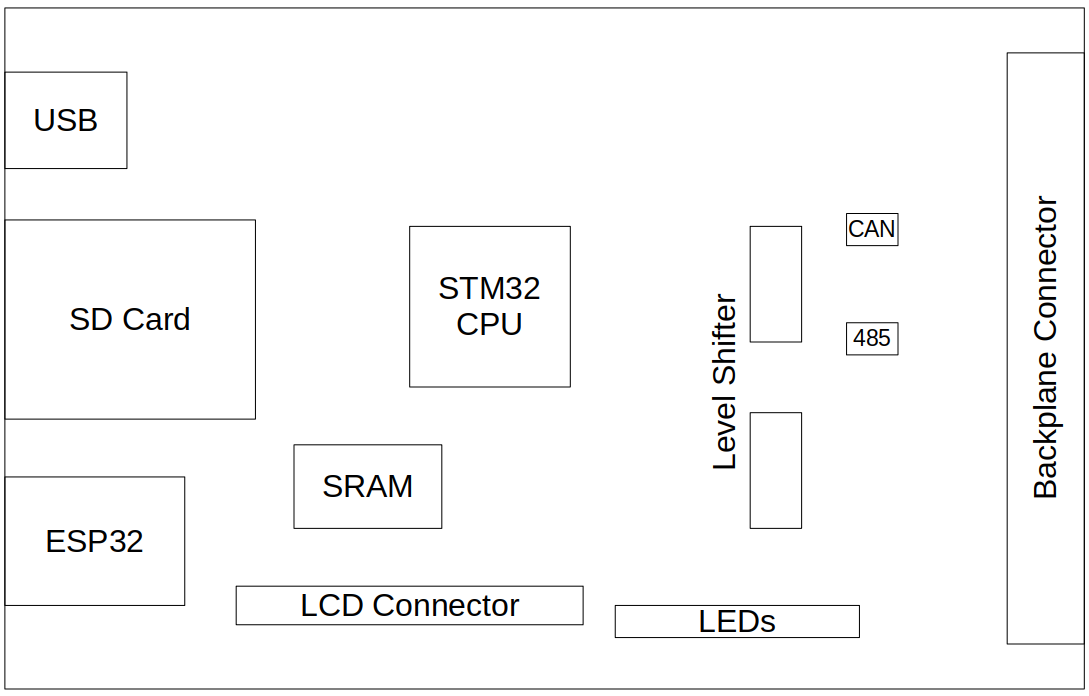
\includegraphics[width=\textwidth]{pictures/overview_cpu.png}
	\caption{PCB Overview HBC}
	\label{img:HBC}
\end{figure}

\subsection{CPU}

The core of the HBC is the STM32F767 microcontroller. It controls everything in the entire system and provides the user interfaces. 

With 2MB of Flash and 512kB RAM it has more than plenty of storage both for the program code as well as process data and variables. Also at 216MHz max clock rate it is really fast and can process everything in a timely manner. At least that was the thought behind choosing this chip. 

\subsection{Additional Hardware}

Also it has a lot of interfaces which are used on the PCB. Additionally to the interfaces mentioned in chapter 5.4, internally the module has two SPI busses, one for the touch controller and one for the ESP32 coprocessor. A USB interface for debugging and monitoring is inlcuded as well. 

For logging and config storage I included an SD card slot. 

The FSMC (Flexible SRAM Memory Controller) interface of the microcontroller is connected to an external 512k x 16 SRAM chip. I thought about including an external flash memory for application software, but decided against it, since the internal flash seemed more than enough. The external SRAM might come in handy tho if I decide to build modules like logic analyzers which have a ton of data coming in at once. 

The ESP32 module will provide a webinterface for monitoring and diagnosis, but not for controlling the system. This decision was made from a security stand point. 

For Interfacing with the whole system, a 5" Nextion TFT LCD is connected via UART. 

How the protocols on the interfaces will look like, will be discussed in another chapter. 

%------------------------------------------------------------------------------------------------------------------------

\section{Diode Tester}
The Diode Tester is actually quite simple in design. It consists of 4 constant current sources which are tuned to about 2.2mA, 5mA, 10mA and 20mA respectively. Due to this I can enable up to 16 different currents through the Device Under Test (DUT) and even make a crude characteristic curve out of it. 
Following is a simplified schematic of the current sources.

\begin{figure}[H]
	\centering
		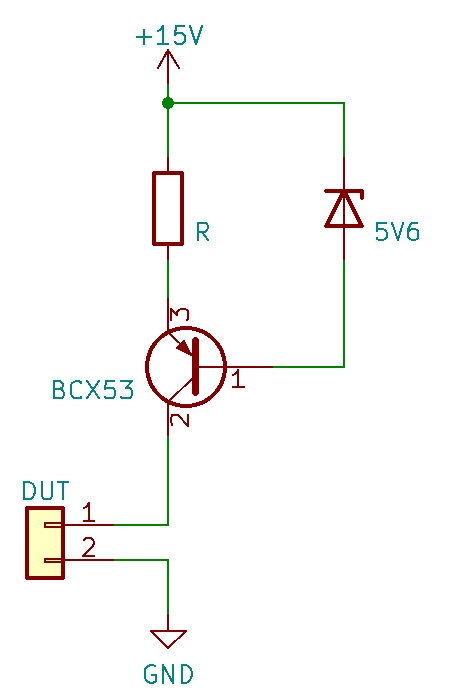
\includegraphics[width=5cm]{pictures/cc_source.png}
	\caption{Current Source Schematic}
	\label{img:CC_Diode}
\end{figure}

The current is configured via the resistor according to Kirchhoff's loop rule. $U_{be}$ of the transistor is typically 0.7V, which means the voltage across the resistor is fixed at $5.6V - 0.7V = 4.9V$. With the values of 2.2k, 1k, 499 and two 499 in parallel respectively, the following currents are available:

\begin{align*}
	\frac{4.9V}{2.2 k\Omega} & = 2.22 mA\\
	\frac{4.9V}{1 k\Omega}  & = 4.9  mA\\
	\frac{4.9V}{499 \Omega} & = 9.81 mA\\
	\frac{4.9V}{249.5 \Omega} & = 19.63 mA\\
\end{align*}

In V1 I tried to enable the sources via a P-channel MOSFET, which for some strange reason didn't work. So I decided for V2 to use small reed relais I had in storage. 

\vspace{1cm}

The module also has an STM32F103 controller on board which is connected to the backplane via CAN and I2C. I did both since I hadn't yet decided which interface I am going to use for the module. 

\subsection{Parameters}
\begin{table}[H]
    \centering
    \begin{tabular}{|c|c|l|}
        \hline
        \textbf{No.}   &   \textbf{Size} & \multicolumn{1}{|c|}{\textbf{Description}}\\ \hline \hline
        10h   &  2 Byte & DUT Voltage at 2 mA \\ \hline
		11h   &  2 Byte & DUT Voltage at 5 mA \\ \hline
		12h   &  2 Byte & DUT Voltage at 7 mA \\ \hline
		13h   &  2 Byte & DUT Voltage at 10 mA \\ \hline
		14h   &  2 Byte & DUT Voltage at 12 mA \\ \hline
		15h   &  2 Byte & DUT Voltage at 15 mA \\ \hline
		16h   &  2 Byte & DUT Voltage at 17 mA \\ \hline
		17h   &  2 Byte & DUT Voltage at 20 mA \\ \hline
		18h   &  2 Byte & DUT Voltage at 22 mA \\ \hline
		19h   &  2 Byte & DUT Voltage at 25 mA \\ \hline
		1Ah   &  2 Byte & DUT Voltage at 27 mA \\ \hline
		1Bh   &  2 Byte & DUT Voltage at 30 mA \\ \hline
		1Ch   &  2 Byte & DUT Voltage at 32 mA \\ \hline
		1Dh   &  2 Byte & DUT Voltage at 35 mA \\ \hline
		1Eh   &  2 Byte & DUT Voltage at 37 mA \\ \hline
		20h   &  1 Byte & Starting Current	\\ \hline
		21h   &  1 Byte & Ending Current \\ \hline
    \end{tabular}
	\caption{Diode Tester Parameter List}
\label{tab:Par-Diode}
\end{table}
\subsection{Operation Modes}
Start Measurement with ``Enable Output'' Command.

\begin{table}[H]
    \centering
    \begin{tabular}{|c|c|l|}
        \hline
        \textbf{Mode}   &  \multicolumn{1}{|c|}{\textbf{Description}}\\ \hline \hline
        0   &  \makecell[l]{Single Value Measurement \\ Starting Current only}\\ \hline
		1   &  \makecell[l]{Coarse Characteristic Curve \\ Starting Current to Ending Current \\ Only Hardware Sources enabled}\\ \hline
		2   &  \makecell[l]{Medium Characteristic Curve \\ Starting Current to Ending Current \\ Every other possible current}\\ \hline
		3   &  \makecell[l]{Fine Characteristic Curve \\ Starting Current to Ending Current \\ Every possible current}\\ \hline
    \end{tabular}
	\caption{Diode Tester Parameter List}
\label{tab:Modes-Diode}
\end{table}
\subsection{Channels/Outputs}
Enabled Channels:
\begin{itemize}
	\item ADC0
\end{itemize}
\section{Waveform Generator DDS}
For most of the design I have to thank ``Daumemo'' from \textcolor{blue}{\href{https://daumemo.com}{daumemo.com}}. I wanted to use the AD9833 waveform generator IC and his guide helped me design the circuit around it. 

The board mainly consists of the STM32F103 controller, the AD9833 signal generator, a VCA (voltage controlled amplifier) and an output amplifier. Gain and Offset are controlled via PWM, the Interface to the AD9833 is SPI. 

The Signal Generator is capable of generating Sine, Triangle and Square waves from 0.1Hz up to 12.5MHz with a 0.1Hz resolution. 

\vspace{1cm}

I will add more info once I get to program the module. 

\subsection{Parameters}
\subsection{Operation Modes}
\subsection{Channels/Outputs}
\section{Symmetric Linear Power Supply (SymPSU)}
The design for the symmetric power supply is derived from the user ``The Big One'' over on \textcolor{blue}{\href{https://hackaday.io/project/4154-bench-power-supply}{Hackaday}}. I adopted it to my STM32 controller and to 3V3 supply voltage. Also I switched the control voltage generation from a dedicated DAC to the PWM-channels of the STM32. I am using the internal ADC on the STM32 as well. 

With these design changes, the SymPSU can provide the following voltages:
\begin{itemize}
	\item Positive voltage
	\begin{itemize}
		\item 0 to 12V @ 0 to 1.2A
	\end{itemize}
	\item Negative voltage
	\begin{itemize}
		\item 0 to -12V @ 0 to 1.2A
	\end{itemize}
\end{itemize}

After tweaking the code, I programmed the following resolutions:

\begin{itemize}
	\item Voltages
	\begin{itemize}
		\item 10 mV / step
	\end{itemize}
	\item Currents
	\begin{itemize}
		\item 0.1 mA / step
	\end{itemize}
\end{itemize}

I am quite happy with these specs, but will likely tweak the design in the future a bit. I still have some issues that are currently fixed in software, rather than in hardware. 

\subsection{Parameters}
\begin{table}[H]
    \centering
    \begin{tabular}{|c|c|l|}
        \hline
        \textbf{No.}   &   \textbf{Size} & \multicolumn{1}{|c|}{\textbf{Description}}\\ \hline \hline
        10h   &  2 Byte &  Set Positive Voltage [mV]\\ \hline
		11h   &  2 Byte &  Set Positive Current [mA]\\ \hline
		12h   &  2 Byte &  Set Negative Voltage [mV]\\ \hline
		13h   &  2 Byte &  Set Negative Current [mA]\\ \hline
		20h   &  2 Byte &  Measured Positive Voltage [mV]\\ \hline
		21h   &  2 Byte &  Measured Positive Current [mA]\\ \hline
		22h   &  2 Byte &  Measured Negative Voltage [mV]\\ \hline
		23h   &  2 Byte &  Measured Negative Current [mA]\\ \hline
    \end{tabular}
	\caption{SymPSU Parameter List}
\label{tab:Par-SymPSU}
\end{table}
\subsection{Operation Modes}
n/a.
\subsection{Channels/Outputs}
Enabled Channels:
\begin{itemize}
	\item ADC0
	\item ADC1
	\item ADC2
	\item ADC3
	\item PWM0
	\item PWM1
	\item PWM2
	\item PWM3
	\item Output Relais
\end{itemize}

\section{Switching Mode Power Supply}
This Power Supply is based on a TL494 PWM Control Circuit. The PWM Controller is getting the reference voltages for Output Voltage and Current from the STM32 via filtered PWM signals. This way a complicated and possibly slow and inaccurate software PID regulator is avoided while the circuit complexity is held at a minimum. A voltage divider is generating the feedback voltage, while a high-current shunt and differential amplifier is generating the feedback voltage for the current. 

The following specs were set for Rev 1. This module will need a redesign in order to fix some mistakes.

\begin{itemize}
	\item Voltage
	\begin{itemize}
		\item 2 .. 22 V Output
		\item 10 mV resolution
	\end{itemize}
	\item Current
	\begin{itemize}
		\item 0 .. 5 A Output
		\item 10 mA resolution
	\end{itemize}
\end{itemize}

\subsection{Parameters}
\begin{table}[H]
    \centering
    \begin{tabular}{|c|c|l|}
        \hline
        \textbf{No.}   &   \textbf{Size} & \multicolumn{1}{|c|}{\textbf{Description}}\\ \hline \hline
        10h   &  2 Byte &  Set Voltage [10mV]\\ \hline
		11h   &  2 Byte &  Set Current [10mA]\\ \hline
		20h   &  2 Byte &  Measured Voltage [10mV]\\ \hline
		21h   &  2 Byte &  Measured Current [10mA]\\ \hline
    \end{tabular}
	\caption{SMPS Parameter List}
\label{tab:Par-SMPS}
\end{table}

\subsection{Operation Modes}
n.a.
\subsection{Channels/Outputs}
Enabled Channels:
\begin{itemize}
	\item ADC0
	\item ADC1
	\item PWM0
	\item PWM1
	\item Output Relais
\end{itemize}				\newpage 	% Modules
\chapter{Interface Protocols}
As the system is quite big and has a lot of interfaces, here will be the place to discuss all these. 

Mainly the USB-Interface, SPI-Interface for the ESP32-Communication and CAN-Interface are of interest. But also the secondary I2C and general SPI interfaces will be defined here. 

\section{USB Monitor}
\textbf{\textcolor[HTML]{FF0000}{TBD}}

USB is currently only used to log the CAN traffic of the system, if the debug-option on the display is set. This will be expanded in the future by a complete USB monitor which will have many different capabilities such as sending CAN frames, setting variables inside the Mainboard and basically letting the ModLab be controlled via USB. 

More on this will be a subject for the future tho. 			\newpage	% Protocol
\section{CAN}
\subsection{Overview}
The CAN bus is the main communication bus for the ModLab. The HBC is sequentially talking to all the connected modules and sending commands to them if needed. This includes regular status updates as well as configurations. The CAN bus itself is divided into seperate layers, which will be discussed now. 

\begin{enumerate}
    \item \textbf{Physical Layer}\\
    The physical layer of the CAN interface consists of the CAN module on the STM32 controllers as well as a SN65VHD232 CAN Transceiver. CAN Rx and TX are sent on the same differential interface, making the bus half-duplex. 

    In order to get enough data around in a feasable time, the Interface will be clocked at 1MHz speed. 
    \item \textbf{Transport Layer}\\
    The transport layer descibes the way the data will be sent. Since standard CAN frames can only handle 8 bytes at once, I thought about implementing something here, to increase the data transfer. 
    
    After careful thinking tho, I decided agains a special transport protocol like ISO-TP, because the overhead creates more delays than I am comfortable with. I just have to be careful designing the command structure to not include commands with too many arguments.

    \item \textbf{Application Layer}\\
    Here is, where it gets interesting. After we can now send plenty of data, I need to define the actual transmission protocol of the payload for the modules. Since CAN is designed as such that every node reads the data at the same time, I have to implement a procedure to let the modules decide if the received message is of interest for them or not. 

    This can be achieved with two different methods. One is by encoding the module address in the ID section of the module, the other is sending the module in question as first byte in the payload. 

    I decided to implement the first option to save on transmission time. The ID field in the datagrams will be used both for encoding the module address, as well as indicaton for special cases like warnings and errors in my protocol. Also with this method I can selectively talk to each module without blocking processing time for checking if the message is really meant for them. 

    To clarify: if I talk about address, I mean the module address. I will refer to the ID as a whole (address + Message Type) as ID.
\end{enumerate}

\newpage

\subsection{General Structure}
The general structure of the protocol uses a ping---pong approach. The command value sent to the module will always be returned to the sender as well to clarify that this is the reply tho this command. Even tho I might sacrifice some bandwidth with this method, I think it will be worthwhile in future implementations. 

Because of this, the structure is always ``Command --- Value'' in both directions.

\subsection{ID Endcoding}
The ID structure will be used as specified in the following table. The ``xx'' in the ID will be placeholders for the module address. 

\begin{table}[H]
    \centering
    \begin{tabular}{|c|l|}
        \hline
        \textbf{ID}   &   \multicolumn{1}{|c|}{\textbf{Type}}\\ \hline \hline
        7xxh   &   Auto Message (informational) \\ \hline
        6xxh   &   Reply to Command (ACK)  \\  \hline
        5xxh   &   Standard Command    \\ \hline
        4xxh   &   Warnings / State Changes\\ \hline
        3xxh   &   Reply to Command (NACK) \\  \hline
        2xxh   &   Processing Error    \\ \hline
        1xxh   &   Critical Error      \\ \hline
        0xxh   &   reserved \\ \hline
    \end{tabular}
    \caption{CAN-Messages}
    \label{tab:CAN-Messages}
\end{table}

\subsection{Auto-Messages}
\textbf{\textcolor[HTML]{FF0000}{TBD}}

\subsection{Base-Addresses}
\begin{table}[H]
    \centering
    \begin{tabular}{|c|l|}
        \hline
        \textbf{Base Address}   &   \multicolumn{1}{|c|}{\textbf{Module}}\\ \hline \hline
        10h    &   HBC    \\ \hline
        20h    &   Diode Tester \\ \hline
        30h    &   Symmetrical Linear Power supply \\ \hline
        34h    &   reserved \\ \hline
        38h    &   reserved \\ \hline
        3Ch    &   24V Switching Mode Power Supply \\\hline
        40h    &   DDS Waveform Generator \\ \hline
    \end{tabular}
    \caption{CAN Addresses}
    \label{tab:CAN-ADD}
\end{table}

\newpage

\subsection{Commands}
Overview:
\begin{table}[H]
    \centering
    \begin{tabular}{|c|l|}
        \hline
        \textbf{Value}   &   \multicolumn{1}{|c|}{\textbf{Command}}\\ \hline \hline \hline
        01h    &   Reset Module \\ \hline

        \hline
        10h    &   Set 8bit Parameter    \\ \hline
        11h    &   Get 8bit Parameter     \\ \hline
        14h    &   Set 16bit Parameter   \\ \hline
        15h    &   Get 16bit Parameter    \\ \hline 
        \hline
        20h    &   Get Status Information \\ \hline 
        \hline
        40h    &   Enable Output       \\ \hline
        41h    &   Disable Output      \\ \hline 
        \hline
        60h    &   Set Operation Mode  (TBD)\\ \hline
        61h    &   Get Operation Mode  (TBD)\\ \hline 
    \end{tabular}
    \caption{CAN-Commands}
\label{tab:CAN-Commands}
\end{table}

%-------------------------------
\subsubsection{10h --- Set 8bit Parameter}
Write 8bit value to module parameter. 

Command:
\begin{table}[H]
    \centering
    \begin{tabular}{|c|c|l|}
        \hline
        \textbf{Value}   &   \textbf{Length} & \multicolumn{1}{|c|}{\textbf{Description}}\\ \hline \hline
        10h   &  1 Byte & Set 8bit Parameter Command \\ \hline
        Index & 1 Byte  & Parameter Index, see Module Description \\ \hline
        Value & 1 Byte & Value to be written\\ \hline
    \end{tabular}
\label{tab:CAN-10-C}
\end{table}
Reply:
\begin{table}[H]
    \centering
    \begin{tabular}{|c|c|l|}
        \hline
        \textbf{Value}   &   \textbf{Length} & \multicolumn{1}{|c|}{\textbf{Description}}\\ \hline \hline
        10h   &  1 Byte & Set 8bit Parameter Command \\ \hline
        Status & 1 Byte & \makecell[l]{Error-Status in case of NACK \\ Otherwise set to 0\\see Error Descriptions}\\ \hline
    \end{tabular}
\label{tab:CAN-10-R}
\end{table}

%-------------------------------
\subsubsection{11h --- Get 8bit Parameter}
Read 8bit value from module parameter.

Command:
\begin{table}[H]
    \centering
    \begin{tabular}{|c|c|l|}
        \hline
        \textbf{Value}   &   \textbf{Length} & \multicolumn{1}{|c|}{\textbf{Description}}\\ \hline \hline
        11h   &  1 Byte & Get 8bit Parameter Command \\ \hline
        Index & 1 Byte  & Parameter Index, see Module Description \\ \hline
    \end{tabular}
\label{tab:CAN-11-C}
\end{table}
Reply:
\begin{table}[H]
    \centering
    \begin{tabular}{|c|c|l|}
        \hline
        \textbf{Value}   &   \textbf{Length} & \multicolumn{1}{|c|}{\textbf{Description}}\\ \hline \hline
        11h   &  1 Byte & Get 8bit Parameter Command \\ \hline
        Status & 1 Byte & \makecell[l]{Error-Status in case of NACK \\ Otherwise set to 0\\see Error Descriptions}\\ \hline
        Value & 1 Byte & Value to be read; 0 if NACK \\ \hline
    \end{tabular}
\label{tab:CAN-11-R}
\end{table}

%-------------------------------
\subsubsection{14h --- Set 16bit Parameter}
Write 16bit value to module parameter.

Command:
\begin{table}[H]
    \centering
    \begin{tabular}{|c|c|l|}
        \hline
        \textbf{Value}   &   \textbf{Length} & \multicolumn{1}{|c|}{\textbf{Description}}\\ \hline \hline
        14h   &  1 Byte & Set 16bit Parameter Command \\ \hline
        Index & 1 Byte  & Parameter Index, see Module Description \\ \hline
        Value & 2 Byte & Value to be written\\ \hline
    \end{tabular}
\label{tab:CAN-14-C}
\end{table}
Reply:
\begin{table}[H]
    \centering
    \begin{tabular}{|c|c|l|}
        \hline
        \textbf{Value}   &   \textbf{Length} & \multicolumn{1}{|c|}{\textbf{Description}}\\ \hline \hline
        14h   &  1 Byte & Set 16bit Parameter Command \\ \hline
        Status & 1 Byte & \makecell[l]{Error-Status in case of NACK \\ Otherwise set to 0\\see Error Descriptions}\\ \hline
    \end{tabular}
\label{tab:CAN-14-R}
\end{table}
\subsubsection{15h --- Get 16bit Parameter}
Read 16bit value from module parameter.

Command:
\begin{table}[H]
    \centering
    \begin{tabular}{|c|c|l|}
        \hline
        \textbf{Value}   &   \textbf{Length} & \multicolumn{1}{|c|}{\textbf{Description}}\\ \hline \hline
        15h   &  1 Byte & Get 16bit Parameter Command \\ \hline
        Index & 1 Byte  & Parameter Index, see Module Description \\ \hline
    \end{tabular}
\label{tab:CAN-15-C}
\end{table}
Reply:
\begin{table}[H]
    \centering
    \begin{tabular}{|c|c|l|}
        \hline
        \textbf{Value}   &   \textbf{Length} & \multicolumn{1}{|c|}{\textbf{Description}}\\ \hline \hline
        15h   &  1 Byte & Get 16bit Parameter Command \\ \hline
        Status & 1 Byte & \makecell[l]{Error-Status in case of NACK \\ Otherwise set to 0\\see Error Descriptions}\\ \hline
        Value & 2 Byte & Value to be read; 0 if NACK \\ \hline
    \end{tabular}
\label{tab:CAN-15-R}
\end{table}

%-------------------------------
\subsubsection{20h --- Get Status Information}
Get status information from module.

Command:
\begin{table}[H]
    \centering
    \begin{tabular}{|c|c|l|}
        \hline
        \textbf{Value}   &   \textbf{Length} & \multicolumn{1}{|c|}{\textbf{Description}}\\ \hline \hline
        20h   &  1 Byte & Get Status Information Command \\ \hline
    \end{tabular}
\label{tab:CAN-20-C}
\end{table}
Reply:
\begin{table}[H]
    \centering
    \begin{tabular}{|c|c|l|}
        \hline
        \textbf{Value}   &   \textbf{Length} & \multicolumn{1}{|c|}{\textbf{Description}}\\ \hline \hline
        20h   &  1 Byte & Get 16bit Parameter Command \\ \hline
        Status & 1 Byte & \makecell[l]{Error-Status\\see Error Descriptions}\\ \hline
        Channel Info & 1 Byte & \makecell[l]{bit 0..3: PWM-Channel 0..3\\bit 4..5: ADC-Channel 0..3\\bits are 0 if channel not implemented} \\ \hline
    \end{tabular}
\label{tab:CAN-20-R}
\end{table}
%-------------------------------
\subsubsection{40h --- Enable Output}
Enable the Module Output.

Command:
\begin{table}[H]
    \centering
    \begin{tabular}{|c|c|l|}
        \hline
        \textbf{Value}   &   \textbf{Length} & \multicolumn{1}{|c|}{\textbf{Description}}\\ \hline \hline
        40h   &  1 Byte & Enable Output Command \\ \hline
    \end{tabular}
\label{tab:CAN-40-C}
\end{table}
Reply:
\begin{table}[H]
    \centering
    \begin{tabular}{|c|c|l|}
        \hline
        \textbf{Value}   &   \textbf{Length} & \multicolumn{1}{|c|}{\textbf{Description}}\\ \hline \hline
        40h   &  1 Byte & Enable Output Command \\ \hline
        Status & 1 Byte & \makecell[l]{Error-Status\\see Error Descriptions}\\ \hline
    \end{tabular}
\label{tab:CAN-40-R}
\end{table}
%-------------------------------
\subsubsection{41h --- Disable Output}
Disable the Module Output.

Command:
\begin{table}[H]
    \centering
    \begin{tabular}{|c|c|l|}
        \hline
        \textbf{Value}   &   \textbf{Length} & \multicolumn{1}{|c|}{\textbf{Description}}\\ \hline \hline
        41h   &  1 Byte & Disable Output Command \\ \hline
    \end{tabular}
\label{tab:CAN-41-C}
\end{table}
Reply:
\begin{table}[H]
    \centering
    \begin{tabular}{|c|c|l|}
        \hline
        \textbf{Value}   &   \textbf{Length} & \multicolumn{1}{|c|}{\textbf{Description}}\\ \hline \hline
        41h   &  1 Byte & Disable Output Command \\ \hline
        Status & 1 Byte & \makecell[l]{Error-Status\\see Error Descriptions}\\ \hline
    \end{tabular}
\label{tab:CAN-41-R}
\end{table}
%-------------------------------
\subsubsection{60h --- Set Operation Mode}
Set Module into Operation Mode x. 

Command:
\begin{table}[H]
    \centering
    \begin{tabular}{|c|c|l|}
        \hline
        \textbf{Value}   &   \textbf{Length} & \multicolumn{1}{|c|}{\textbf{Description}}\\ \hline \hline
        60h   &  1 Byte & Set Operation Mode Command \\ \hline
        Mode & 1 Byte & Operation Mode, see Module Description\\ \hline
    \end{tabular}
\label{tab:CAN-60-C}
\end{table}
Reply:
\begin{table}[H]
    \centering
    \begin{tabular}{|c|c|l|}
        \hline
        \textbf{Value}   &   \textbf{Length} & \multicolumn{1}{|c|}{\textbf{Description}}\\ \hline \hline
        60h   &  1 Byte & Set Operation Mode Command \\ \hline
        Status & 1 Byte & \makecell[l]{Error-Status in case of NACK \\ Otherwise set to 0\\see Error Descriptions}\\ \hline
    \end{tabular}
\label{tab:CAN-60-R}
\end{table}

\subsubsection{61h --- Get Operation Mode}
Get Module Operation Mode. 

Command:
\begin{table}[H]
    \centering
    \begin{tabular}{|c|c|l|}
        \hline
        \textbf{Value}   &   \textbf{Length} & \multicolumn{1}{|c|}{\textbf{Description}}\\ \hline \hline
        61h   &  1 Byte & Get Operation Mode Command \\ \hline
    \end{tabular}
\label{tab:CAN-61-C}
\end{table}
Reply:
\begin{table}[H]
    \centering
    \begin{tabular}{|c|c|l|}
        \hline
        \textbf{Value}   &   \textbf{Length} & \multicolumn{1}{|c|}{\textbf{Description}}\\ \hline \hline
        61h   &  1 Byte & Get Operation Mode Command \\ \hline
        Mode & 1 Byte & Operation Mode, see Module Description\\ \hline
        Status & 1 Byte & \makecell[l]{Error-Status in case of NACK \\ Otherwise set to 0\\see Error Descriptions}\\ \hline
    \end{tabular}
\label{tab:CAN-61-R}
\end{table}

%-------------------------------


\subsection{Error Descriptions}
\subsubsection{Status Byte}
Description of the Status Byte in Reply Messages. If a Bit is set to 0, it is inactive. A 1 indicates an active error.

The lower Nibble indicates protocol errors, a mismatch condition can mean both ``not available'' and ``wrong length''. 

The upper Nibble indicates internal errors of the module. 

\begin{table}[H]
    \centering
    \begin{tabular}{|c|l|}
        \hline
        \textbf{Bit}   & \multicolumn{1}{|c|}{\textbf{Description}}\\ \hline \hline
        0   &    Index Mismatch   \\ \hline
        1   &    Data Mismatch   \\ \hline
        2   &    Channel Mismatch   \\ \hline
        3   &    Operation Mode Mismatch  \\ \hline
        4   &    Processing Error   \\ \hline
        5   &    I/O Error   \\ \hline
        6   &    Unknown Command   \\ \hline
        7   &    reserved   \\ \hline
    \end{tabular}
\label{tab:CAN-status}
\end{table}

\newpage
\section{ESP SPI}
\textbf{\textcolor[HTML]{FF0000}{TBD}}

\section{Backplane SPI}
\textbf{\textcolor[HTML]{FF0000}{TBD}}
\subsection{5V SPI}
\textbf{\textcolor[HTML]{FF0000}{TBD}}
\subsection{3V3 SPI}
\textbf{\textcolor[HTML]{FF0000}{TBD}}

\section{I2C}
\textbf{\textcolor[HTML]{FF0000}{TBD}}
\subsection{Standard Mode}
\textbf{\textcolor[HTML]{FF0000}{TBD}}
\subsection{Fast Mode}
\textbf{\textcolor[HTML]{FF0000}{TBD}}


% --------------------------------------------------------------------
% abschließende Verzeichnisse
% --------------------------------------------------------------------

\pagestyle{empty}
\vspace*{\fill}
\begin{center}
\hrulefill\\
\vspace{4mm}
	\begin{HUGE}
		\textbf{Addenda}
	\end{HUGE}\\
\hrulefill\\
\end{center}
\vspace*{\fill}
\newpage
\pagestyle{plain}


\appendix
%\input{appendix/.ltx}		\newpage 	% Anhang
%\input{appendix/.ltx}		\newpage 	% Anhang
%\chapter{Anhang Sym-LNT}			
%\textcolor{blue}{\href{https://sites.google.com/site/ddmcintosh2projects/_/rsrc/1339000657272/diy-cv-cc-bench-power-supply/BenchPowerSupplySchematics.jpg}{Vorlage}}\\
%\textcolor{blue}{\href{https://sites.google.com/site/ddmcintosh2projects/diy-cv-cc-bench-power-supply}{Original Site}}\\
%Spannungsteiler für Verstärkungsfaktor $\frac{1}{256}$ \\
%Oversampling für Spannungsvorgabe um auf 16bit zu kommen:\\
%$R2/R1= 2,564 = 10k/3k9 -> R2/R1 = 256,4 = 100k/390$
%
%\chapter{Anhang Power-LNT}
%\textcolor{blue}{\href{https://www.electronics-lab.com/project/ampstrike-battery-powered-bench-power-supply/}{Vorlage}}
%
%
%\chapter{Anhang Oszilloskop}
%Falls Ansatz mit DSO138:\\
%DC/DC-Wandler: R05P209S\\
%Liefert 220mA, mit 78L05 Spannung für ATmega erzeugen.\\
%DSO138 braucht 9V mit 120mA\\
%ADUM 1250 ARZ I2C-Isolator\\
%Trigger-LED für evtl als Sync-Ausgang?
%
%\chapter{Anhang Elekronische Last}
%V 7331G Profilkühlkörper (mindestens)\\
%40mm-Lüfter mit Steuerung dazu\\
%Lastkreis galvanisch getrennt!
%
%max. 5A
%
%100mOhm Shunt, 0,7V Ube = 1,2V\\
%5V auf 1,2V:\\
%Spannungsteiler 10k - (3k0 + 160)\\
%Teilungsverhältnis 10:3,16
%
%100mOhm Shunt, 1,5V Ube = 2V\\
%5V auf 2V:\\
%Spannungsteiler 12k - (1k2 + 6k8)\\
%Teilungsverhältnis 10:8

% --------------------------------------------------------------------
\end{document}
